\documentclass[11pt]{article}
\usepackage[margin=1.05in]{geometry}
\usepackage{amsmath,amssymb,amsthm}
\usepackage{booktabs}
\usepackage{graphicx}
\usepackage{tikz}
\usepackage{pgfplots}
\pgfplotsset{compat=1.18}
\usetikzlibrary{arrows.meta,positioning,shapes.misc}
\usepackage[numbers]{natbib}
\usepackage[colorlinks=true,linkcolor=blue!50!black,citecolor=blue!50!black,urlcolor=blue!50!black]{hyperref}
\usepackage{microtype}

\newtheorem{theorem}{Theorem}[section]
\newtheorem{proposition}[theorem]{Proposition}
\newtheorem{corollary}[theorem]{Corollary}
\newtheorem{lemma}[theorem]{Lemma}
\theoremstyle{definition}
\newtheorem{assumption}[theorem]{Assumption}
\theoremstyle{remark}
\newtheorem{remark}[theorem]{Remark}

\newcommand{\colistream}{\textsc{ColiStream}}
\newcommand{\bd}{B_{\mathrm{d}}}
\newcommand{\bp}{B_{\mathrm{p}}}
\newcommand{\bv}{B_{\mathrm{v}}}

\title{\colistream: A Streaming Execution-Cache Architecture for\\
Mixture-of-Experts Inference on Consumer GPUs}
\author{Brian Dean Ullery}
\date{July 14, 2026}

\begin{document}
\maketitle

\begin{abstract}
Mixture-of-Experts (MoE) language models decouple parameter count from
per-token compute, but their working set still dwarfs consumer GPU memory: a
744B-parameter model activates only ${\sim}40$B parameters per token, yet its
routed experts occupy ${\sim}370$\,GB at 4-bit precision. Existing offloading
systems treat VRAM as \emph{storage} and ask which weights fit; \colistream{}
instead treats the GPU as a \emph{streaming compute device} and VRAM as an
\emph{execution cache} at the top of a managed
SSD$\to$RAM$\to$VRAM$\to$SM hierarchy. Expert weights flow through the
hierarchy as tile-chunked asynchronous DMA; compute is event-driven at
sub-expert granularity, so matrix multiplication begins while later tiles of
the same expert are still on the bus; a two-lane PCIe scheduler gives
speculative prefetch strictly tile-bounded interference with demand traffic;
and a recency-primary, decayed-frequency replacement policy retains
temporally local experts in VRAM. We give a pipeline model with explicit
fill/drain bounds, a closed-form tile-size feasibility window that we fit to
measurements ($R^2{=}0.99$), a proof that frequency-primary replacement
suffers unbounded pollution under working-set turnover (observed as a
$7.6\times$ slowdown before the fix), and a Che-approximation analysis of
expected cache behavior under Zipfian expert routing. Implemented inside the
open-source colibr\`i engine and validated token-exactly against a reference
implementation, \colistream{} sustains 26.6--27.1\,GB/s of cold expert
streaming with compute fully hidden (${\sim}2{,}250$ experts/s) and
${\sim}16{,}000$ experts/s from the warm execution cache on a single RTX
5070~Ti, and is $1.065\times$ faster end-to-end than the optimized CPU expert
path on a deliberately adversarial, disk-bound workload whose theoretical
compute-side ceiling is $1.05\times$.
\end{abstract}

\section{Introduction}

Sparse Mixture-of-Experts architectures~\citep{shazeer2017outrageously,
lepikhin2020gshard,fedus2022switch} scale language models to trillions of
parameters while activating only a small routed subset per token, a design
carried to frontier scale by DeepSeek-V3~\citep{deepseek2024v3} and
GLM-5.2~\citep{glm52report}. This sparsity creates a peculiar systems
opportunity: per-token \emph{compute} fits comfortably on a consumer GPU,
while per-token \emph{weights} do not. GLM-5.2 routes $k{=}8$ of 256 experts
in each of $L{=}75$ MoE layers; at 4-bit precision each expert is
$s\approx18.9$\,MB, so a cold token demands $L\,k\,s\approx11.4$\,GB of expert
weights --- against 16\,GB of VRAM and 370\,GB of model.

The dominant response is \emph{placement}: decide which tensors reside in
VRAM, which in RAM, and which on disk, then compute each tensor where it
lives~\citep{sheng2023flexgen,aminabadi2022deepspeed,ren2021zerooffload}.
The colibr\`i engine~\citep{colibri2026}, on which this work builds,
exemplifies the placement view on CPUs: a RAM LRU cache and a learned pinned
set front a disk-resident expert store, and its documentation explicitly
rejects per-use GPU copies because a synchronous NVMe$\to$VRAM copy ``would
only replace the disk bottleneck with a PCIe bottleneck.''

\colistream{} is the answer to that objection. Its premise is that the copy
is only a bottleneck if it is \emph{synchronous}. If expert weights are
treated as a \emph{stream} --- tile-chunked, double-buffered, event-ordered
--- then storage, RAM, the PCIe link, and the GPU operate as concurrent
pipeline stages, and per-token latency collapses from the \emph{sum} of stage
times toward their \emph{maximum} (Theorem~\ref{thm:pipe}). VRAM stops being
storage and becomes what a register file is to a cache hierarchy: the place
where bytes happen to be at the moment they are consumed.

Concretely, this paper makes the following contributions:
\begin{enumerate}
  \item \textbf{Architecture} (\S\ref{sec:arch}). A VRAM \emph{execution
  cache}: a pool of fixed-size expert slots fed by tile-chunked asynchronous
  DMA on dedicated copy lanes, with per-slot CUDA events splitting each
  expert so gate/up projections compute while the down projection is still
  in flight; a two-phase demand submit that overlaps PCIe transfers with
  disk reads; a tile-granular soft-preemption scheduler for speculative
  traffic; and four prefetch sources (current router, cross-layer router
  lookahead, temporal locality, long-term heat) mapped onto two tiers.
  \item \textbf{Analysis} (\S\ref{sec:analysis}). A deterministic pipeline
  bound with explicit fill/drain terms; a closed-form tile-size feasibility
  window balancing per-copy overhead against preemption latency, fitted to
  hardware measurements; a proof that frequency-primary replacement without
  decay suffers total pollution under working-set turnover, motivating
  \colistream's recency-primary decayed policy; and an expected-hit-rate
  analysis via the Che approximation~\citep{che2002hierarchical} under
  Zipfian expert popularity.
  \item \textbf{Implementation and evaluation} (\S\ref{sec:impl},
  \S\ref{sec:eval}). A complete implementation inside
  colibr\`i~\citep{colibri2026} (CUDA backend + engine integration,
  ${\sim}900$ lines), validated \emph{token-exactly} against a reference
  transformer implementation, with a fallback lattice in which every failure
  degrades to the CPU path rather than to a wrong answer. On an RTX 5070~Ti
  we measure 26.6--27.1\,GB/s sustained cold streaming with compute hidden,
  ${\sim}16{,}000$ experts/s warm, a $7.6\times$ replacement-policy ablation,
  and a carefully controlled end-to-end comparison on the real 744B model,
  including an honest account of two confounds (speculative-decoding
  defaults and greedy-path divergence) that initially inflated the measured
  advantage from $1.065\times$ to $1.48\times$.
\end{enumerate}

\section{Related Work}\label{sec:related}

\paragraph{MoE models.} Sparsely gated expert layers were introduced at scale
by \citet{shazeer2017outrageously} and industrialized by
GShard~\citep{lepikhin2020gshard} and Switch
Transformers~\citep{fedus2022switch}. DeepSeek-V3~\citep{deepseek2024v3}
established the modern frontier recipe --- fine-grained experts, sigmoid
routing with auxiliary-loss-free balancing, multi-token
prediction --- that GLM-5.2~\citep{glm52report} follows.

\paragraph{Offloading systems.} FlexGen~\citep{sheng2023flexgen} formulates
dense-LLM offloading as a scheduling problem over a GPU/CPU/disk hierarchy,
optimizing throughput for large batches;
DeepSpeed-Inference~\citep{aminabadi2022deepspeed} and
ZeRO-Offload~\citep{ren2021zerooffload} stream dense weights past the GPU.
\colistream{} differs in exploiting MoE \emph{selectivity}: only the routed
$k/E$ fraction of each layer crosses the bus, which changes the economics
from ``stream everything every token'' to ``cache what routing repeats.''

\paragraph{MoE offloading.} \citet{eliseev2023fast} cache experts in VRAM
with LRU and speculate on next-layer routing for Mixtral-class models;
MoE-Infinity~\citep{xue2024moeinfinity} traces activation patterns to
prefetch experts; Fiddler~\citep{kamahori2024fiddler} executes cold experts
on the CPU instead of moving them. \colistream{} synthesizes all three ideas
and adds what they lack: sub-expert tile streaming with event-driven partial
compute, an explicit two-lane PCIe scheduler with bounded speculative
interference, a replacement policy derived from a pollution analysis, and a
disk tier below RAM (370\,GB does not fit in RAM, unlike Mixtral).

\paragraph{Caching theory.} Replacement is classical: Belady's optimal
policy~\citep{belady1966study}, LRU-K~\citep{oneil1993lruk}, and
ARC~\citep{megiddo2003arc} inform \S\ref{sec:policy}; the Che
approximation~\citep{che2002hierarchical} underlies our hit-rate model.
Speculative decoding~\citep{leviathan2023fast} and weight
quantization~\citep{frantar2022gptq,dettmers2022llmint8} are orthogonal
levers the implementation composes with.

\section{The \colistream{} Architecture}\label{sec:arch}

\begin{figure}[t]
\centering
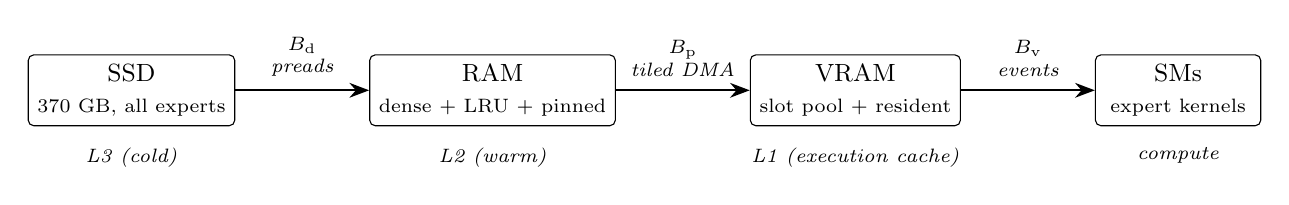
\begin{tikzpicture}[
  tier/.style={draw, rounded corners=2pt, minimum height=9mm, minimum width=21mm, align=center, font=\small},
  lbl/.style={font=\scriptsize\itshape, align=center},
  flow/.style={-{Stealth[length=2.5mm]}, thick}]
\node[tier] (ssd) {SSD\\{\scriptsize 370 GB, all experts}};
\node[tier, right=17mm of ssd] (ram) {RAM\\{\scriptsize dense + LRU + pinned}};
\node[tier, right=17mm of ram] (vram) {VRAM\\{\scriptsize slot pool $+$ resident}};
\node[tier, right=17mm of vram] (sm) {SMs\\{\scriptsize expert kernels}};
\draw[flow] (ssd) -- node[lbl,above=0.5mm]{$\bd$\\preads} (ram);
\draw[flow] (ram) -- node[lbl,above=0.5mm]{$\bp$\\tiled DMA} (vram);
\draw[flow] (vram) -- node[lbl,above=0.5mm]{$\bv$\\events} (sm);
\node[lbl, below=1.5mm of ssd] {L3 (cold)};
\node[lbl, below=1.5mm of ram] {L2 (warm)};
\node[lbl, below=1.5mm of vram] {L1 (execution cache)};
\node[lbl, below=1.5mm of sm] {compute};
\end{tikzpicture}
\caption{The \colistream{} hierarchy. Every level behaves as a cache over the
level below; no expert permanently occupies VRAM except a measured hot set.}
\label{fig:hier}
\end{figure}

\subsection{Design premise}
Traditional GPU inference asks: \emph{which weights fit in VRAM?}
\colistream{} asks: \emph{is every hardware engine --- NVMe queue, PCIe copy
engine, tensor pipeline --- busy at every instant?} VRAM is a high-speed
execution cache, not permanent storage (Fig.~\ref{fig:hier}). The
scheduler's objective is that the compute units never stall on memory unless
prediction fails \emph{and} every faster tier misses.

\subsection{Expert representation and tile streaming}\label{sec:tiles}
Each routed expert comprises three quantized matrices (gate, up, down
projections) plus per-row scales, stored contiguously. Rather than treating
the expert as the unit of transfer, \colistream{} streams it as a sequence of
fixed-size \emph{tiles} ($t = 512$\,KB by default, configurable
64\,KB--4\,MB via \texttt{--stream-tile-kb}). Tiles serve two purposes:
\begin{enumerate}
\item \textbf{Partial-compute overlap.} Two CUDA events split each expert:
one after the gate/up matrices (two-thirds of the bytes, transferred first),
one after the down matrix. The gate/up kernels and the SiLU are enqueued
against the first event, the down kernel against the second --- so
computation of an expert begins while its own tail is still on the bus.
\item \textbf{Soft preemption.} A tile is the scheduling quantum of the PCIe
link (\S\ref{sec:pcie}): the worst-case delay a demand transfer suffers
behind speculative traffic is one tile, not one expert.
\end{enumerate}

\subsection{The VRAM execution cache}
VRAM is carved into $C$ fixed-size slots ($C{=}727$ at 18.9\,MB on a 16\,GB
card after the dense reserve), each holding one expert keyed by (layer,
expert). Fixed slots eliminate fragmentation and make transfer cost uniform,
which in turn drops the transfer-cost term out of replacement comparisons.
Slots carry busy bits (in-flight demand groups, in-flight uploads) so
eviction can never race an active consumer, and per-slot events make reuse
ordering explicit. Container quantization formats (int8; int4 offset-nibble;
int2; f32) are decoded \emph{inside} the kernels, so any mixture streams
as-is with no conversion pass.

\subsection{Execution pipeline and double buffering}
A MoE layer's demand set (the $k$ routed experts per position, deduplicated
batch-wide) is submitted split-phase. Phase~0 submits RAM-resident experts
immediately: their DMA and kernels run \emph{while} the I/O pool is still
reading the disk misses. Phase~1 submits the misses as their preads land.
Within a phase, cache \emph{hits} are enqueued before \emph{misses}, so a
resident expert never queues behind another expert's transfer. All kernels
issue to one execution stream; all demand DMA to a dedicated copy stream ---
while the GPU computes expert $j$, the copy engine fills expert $j{+}1$'s
slot. Classical A/B double buffering is the $C{=}2$ special case; the slot
pool generalizes the same overlap across an entire layer plus prefetch depth.
The host thread regains control immediately after enqueue (split-phase
begin/end), so the CPU runs the shared expert and attention of the next
layer concurrently with the GPU pipeline.

\begin{figure}[t]
\centering
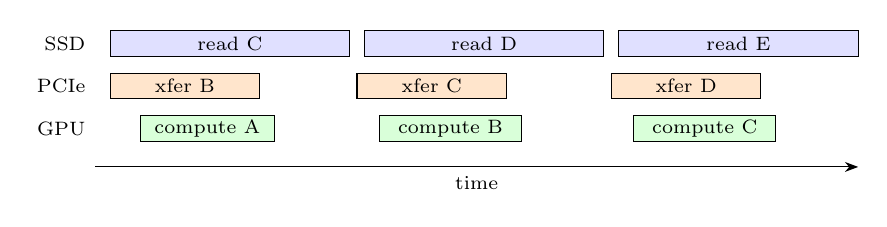
\begin{tikzpicture}[x=0.95mm, y=5.4mm, font=\scriptsize]
% rows: SSD, PCIe, GPU
\node[anchor=east] at (0,2) {SSD};
\node[anchor=east] at (0,1) {PCIe};
\node[anchor=east] at (0,0) {GPU};
% SSD reads
\foreach \s/\e/\n in {2/34/C, 36/68/D, 70/102/E}
  \draw[fill=blue!12] (\s,1.7) rectangle node{read \n} (\e,2.3);
% PCIe transfers
\foreach \s/\e/\n in {2/22/B, 35/55/C, 69/89/D}
  \draw[fill=orange!20] (\s,0.7) rectangle node{xfer \n} (\e,1.3);
% GPU compute
\foreach \s/\e/\n in {6/24/A, 38/57/B, 72/91/C}
  \draw[fill=green!15] (\s,-0.3) rectangle node{compute \n} (\e,0.3);
\draw[-{Stealth}] (0,-0.9) -- node[below]{time} (102,-0.9);
\end{tikzpicture}
\caption{Steady-state timeline. Disk reads expert $n{+}2$, PCIe transfers
$n{+}1$, and the GPU computes $n$, concurrently; each engine's idle time is
bounded by the pipeline imbalance, not by the sum of the other stages.}
\label{fig:timeline}
\end{figure}

\subsection{The PCIe scheduler}\label{sec:pcie}
Two copy lanes share the link. Demand groups own a high-priority stream.
Speculative uploads (below) ride a second stream and \emph{yield between
tiles} whenever a demand group is active: since hardware copy queues are
FIFO and in-flight copies cannot be aborted~\citep{nvidia2025cuda},
tile-granular yielding is the practical form of preemption, with
interference bounded by Proposition~\ref{prop:tile}. Stale speculative work
is cancelled at the queue, the only place cancellation is possible.

\subsection{Prefetch sources}\label{sec:prefetch}
Four signals keep the queue full, in priority order:
\begin{enumerate}
\item \textbf{Current router} --- the demand path itself.
\item \textbf{Layer predictor} --- applying layer $\ell{+}1$'s router to
layer $\ell$'s post-attention state recalls 71.6\% of the true top-8
(measured by colibr\`i~\citep{colibri2026}); a pilot thread loads predicted
experts from disk and pushes them into the execution cache over the
speculative lane \emph{while it still exclusively owns the host buffer},
eliminating use-after-recycle races by construction.
\item \textbf{Temporal locality} --- handled by retention rather than
transfer: experts used for token $n$ remain cached for token $n{+}1$
(\S\ref{sec:policy}), so the characteristic ``4\,4\,7\,4\,4\,7'' repetition
of MoE routing becomes zero-traffic hits.
\item \textbf{Long-term heat} --- persistent routing histograms place the
globally hot set as \emph{resident} tensors at startup (colibr\`i's learned
pin), a tier \colistream{} deliberately preserves: the streaming cache
serves the tail, not the head.
\end{enumerate}
Because the execution cache sits \emph{above} RAM, residency is probed at
routing time: an expert present in VRAM but evicted from RAM skips its disk
read entirely.

\subsection{Replacement policy}\label{sec:policy}
Each slot carries a decayed frequency $f$ and a last-use clock $r$. The
victim minimizes the score
\begin{equation}
\sigma(\text{slot}) \;=\; \big(\min(2^{16}{-}1,\;\text{recency})\big)\!\ll\!16
\;\big|\;\min(2^{16}{-}1, f),
\qquad f \leftarrow \lfloor f/2 \rfloor \text{ every } C \text{ evictions},
\label{eq:score}
\end{equation}
i.e.\ \emph{recency-primary with frequency tiebreak and periodic decay}.
This inverts the frequency-primary LFRU used by colibr\`i's RAM hot store,
deliberately: \S\ref{sec:pollution} proves that frequency-primary scoring
self-destructs under working-set turnover, and \S\ref{sec:eval} measures the
failure at $7.6\times$. The division of labor is principled --- long-term
frequency belongs to the resident tier (source 4 above); the streaming
cache's dominant signal is the temporal locality of the demand stream itself.

\subsection{Failure containment}
Every stage degrades to the host path, never to a wrong answer: an
oversized expert (e.g.\ the int8 multi-token-prediction head) is rejected
per-expert via an acceptance mask; a group whose synchronization fails is
recomputed on the CPU from host buffers whose lifetime provably spans the
group; a failed speculative upload simply forgets the prediction; a stale
residency probe is caught by a null-buffer guard and falls back to a fresh
disk read. Output correctness never depends on the cache, the scheduler, or
the predictor being right.

\section{Analysis}\label{sec:analysis}

\subsection{Notation and model}
A token demands $M$ expert applications per MoE layer ($M \le k \cdot
\text{batch}$ after deduplication). Each expert has size $s$ bytes. Demand
misses cascade: a VRAM hit costs only kernel time $c$; a RAM hit crosses
PCIe at bandwidth $\bp$; a full miss is first read from disk at $\bd$.
Let $h_V$ be the VRAM hit rate and $h_R$ the conditional RAM hit rate given
a VRAM miss. Per layer,
$M_p = M(1-h_V)$ experts cross PCIe and $M_d = M(1-h_V)(1-h_R)$ come from
disk. We write $\tau$ for the service time of one tile at the slowest stage
and $m$ for the number of pipeline stages ($m{=}3$: disk, PCIe, compute).

\begin{proposition}[Serial cost]\label{prop:serial}
A load-then-execute engine that fetches and computes each expert
synchronously spends, per layer,
\begin{equation}
T_{\mathrm{serial}} \;=\; M_d\,\frac{s}{\bd} \;+\; M_p\,\frac{s}{\bp}
\;+\; M\,c .
\end{equation}
\end{proposition}
\begin{proof}
Immediate: with no overlap, stage times add per expert, and experts add per
layer.
\end{proof}

\begin{assumption}\label{ass:pipe}
(i) The three stages run on independent engines (NVMe queue, DMA copy
engine, SMs); (ii) each stage is work-conserving and FIFO within a demand
group; (iii) at least two slots of buffering separate consecutive stages
(double buffering); (iv) every transfer and read is decomposed into tiles of
service time at most $\tau$ per stage.
\end{assumption}

\begin{theorem}[Pipeline bound]\label{thm:pipe}
Under Assumption~\ref{ass:pipe}, the per-layer completion time of the
streamed pipeline satisfies
\begin{equation}
T_{\mathrm{stream}} \;\le\;
\max\!\Big( M_d\,\frac{s}{\bd},\;\; M_p\,\frac{s}{\bp},\;\; M\,c \Big)
\;+\; (m-1)\,\tau .
\end{equation}
\end{theorem}
\begin{proof}
Index the $N$ tiles of the layer's demand set in FIFO order and let
$\tau_j^{(i)}$ be tile $i$'s service time at stage $j$, with stage busy
times $\beta_j=\sum_i \tau_j^{(i)}$ (so $\beta_1 = M_d s/\bd$, $\beta_2 =
M_p s/\bp$, $\beta_3 = M c$ up to per-tile rounding absorbed into $\tau$).
Let $F_j^{(i)}$ be tile $i$'s finish time at stage $j$. With
work-conservation and sufficient buffering,
$F_j^{(i)} = \max\big(F_j^{(i-1)},\, F_{j-1}^{(i)}\big) + \tau_j^{(i)}$.
By induction on $(i,j)$,
$F_j^{(i)} \le \max_{j'\le j}\big(\sum_{i'\le i}\tau_{j'}^{(i')}\big)
+ \sum_{j'<j}\max_i \tau_{j'}^{(i)}$:
the first term is bounded by the largest partial busy time, and each stage
boundary contributes at most one maximal tile of fill delay. Evaluating at
$i=N$, $j=m$ gives
$T_{\mathrm{stream}} = F_m^{(N)} \le \max_j \beta_j + (m-1)\tau$.
\end{proof}

\begin{corollary}[Streaming speedup]\label{cor:speedup}
Ignoring the $O(m\tau)$ fill term, streaming converts the sum of stage times
into their maximum:
$\;T_{\mathrm{serial}}/T_{\mathrm{stream}} \to
\big(\sum_j \beta_j\big)/\max_j \beta_j \in [1, m]$,
maximized when stages are balanced. Conversely, when one stage dominates
(e.g.\ $\beta_1 \gg \beta_2 + \beta_3$, a slow disk), \emph{no} improvement
to the other stages can exceed the Amdahl bound~\citep{amdahl1967validity}
$T_{\mathrm{serial}}/\beta_1 = 1/\varphi$ where $\varphi = \beta_1 /
T_{\mathrm{serial}}$.
\end{corollary}

With the measured parameters of our evaluation platform ($\bd \approx
0.5$\,GB/s, $\bp \approx 27$\,GB/s pinned, $s=18.9$\,MB, $M=600$ per token
cold), $\beta_1 \approx 22.7$\,s $\gg \beta_2 \approx 0.42$\,s $\gg \beta_3$:
cold decode is disk-bound by a factor of 50, and 10--20\% CPU/GPU utilization
is the \emph{correct} signature of a saturated pipeline, not a defect.
The tier's leverage grows exactly as $h_V, h_R \to 1$ move $\beta_1$ off the
critical path; the warm limit is $\max(\beta_2,\beta_3)$, measured in
\S\ref{sec:micro} at ${\sim}16{,}000$ experts/s.

\subsection{Tile size: overhead vs.\ preemption}\label{sec:tilesize}
Let $c_t$ be the fixed cost of issuing one tile (API call, WDDM submission,
copy-engine descriptor) and $B_\infty$ the asymptotic link bandwidth. An
expert of $s$ bytes in tiles of $t$ bytes transfers in time
\begin{equation}
T(t) = \frac{s}{B_\infty} + \Big\lceil \frac{s}{t} \Big\rceil c_t
\qquad\Longrightarrow\qquad
B_{\mathrm{eff}}(t) = \frac{B_\infty}{1 + c_t B_\infty / t},
\label{eq:beff}
\end{equation}
while a demand transfer arriving behind speculative traffic waits at most
$W(t) = t/B_\infty + c_t$.

\begin{proposition}[Feasible tile window]\label{prop:tile}
For overhead fraction at most $\varepsilon$ and preemption delay at most
$\delta$, the tile size must satisfy
\begin{equation}
\frac{c_t B_\infty (1-\varepsilon)}{\varepsilon} \;\le\; t \;\le\;
B_\infty(\delta - c_t).
\end{equation}
The window is nonempty iff $\delta \ge c_t/\varepsilon$ (up to the
$(1{-}\varepsilon)$ factor); both bounds scale linearly in $B_\infty$, so
faster links want proportionally larger tiles.
\end{proposition}
\begin{proof}
Directly from $B_{\mathrm{eff}}(t) \ge (1-\varepsilon)B_\infty$ and
$W(t)\le\delta$ in \eqref{eq:beff}.
\end{proof}

Fitting \eqref{eq:beff} by least squares to measured per-expert transfer
times at $t \in \{0.5, 2, 4\}$\,MB (Fig.~\ref{fig:tile}) yields $B_\infty =
27.6$\,GB/s and $c_t = 2.0\,\mu$s with $R^2 = 0.99$. At the default
$t=512$\,KB this predicts 90\% of asymptotic bandwidth with $W \le 21\,\mu$s
--- three orders of magnitude below an expert's transfer time, so
speculative traffic is effectively invisible to demand latency.

\begin{figure}[t]
\centering
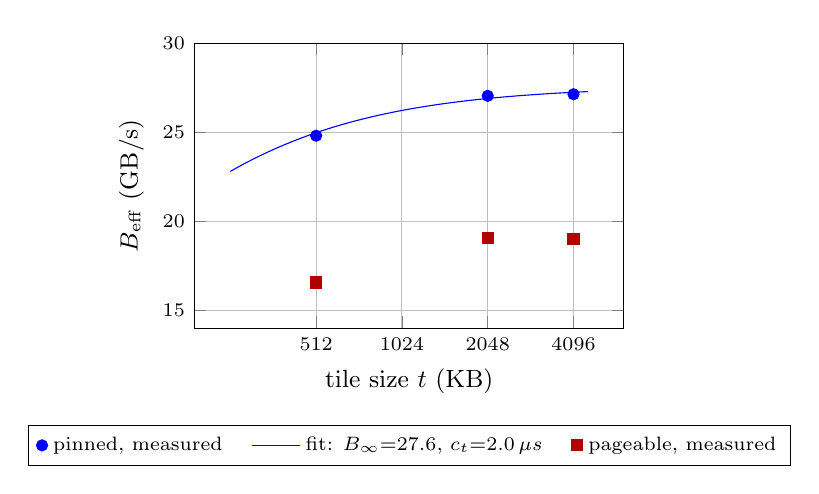
\begin{tikzpicture}
\begin{axis}[width=0.58\textwidth, height=52mm,
  xlabel={tile size $t$ (KB)}, ylabel={$B_{\mathrm{eff}}$ (GB/s)},
  xmode=log, log basis x=2, xtick={512,1024,2048,4096},
  xticklabels={512,1024,2048,4096},
  ymin=14, ymax=30,
  legend style={font=\scriptsize, at={(0.5,-0.34)}, anchor=north, legend columns=3,
    /tikz/every even column/.append style={column sep=3mm}},
  grid=major, tick label style={font=\scriptsize}, label style={font=\small}]
\addplot[only marks, mark=*, blue] coordinates {(512,24.80) (2048,27.04) (4096,27.13)};
\addlegendentry{pinned, measured}
\addplot[blue, domain=256:4608, samples=60]
  {27.6/(1 + 2.0e-6*27.6e9/(x*1024))};
\addlegendentry{fit: $B_\infty{=}27.6$, $c_t{=}2.0\,\mu s$}
\addplot[only marks, mark=square*, red!70!black] coordinates {(512,16.56) (2048,19.05) (4096,18.99)};
\addlegendentry{pageable, measured}
\end{axis}
\end{tikzpicture}
\caption{Effective streaming bandwidth vs.\ tile size on PCIe 5.0 x16
under Windows/WDDM (RTX 5070 Ti), with the two-parameter overhead model of
Eq.~\eqref{eq:beff}. Page-locked host memory buys ${\sim}1.45\times$ over
pageable; the WDDM submission path, not the wire, sets $B_\infty$.}
\label{fig:tile}
\end{figure}

\subsection{Frequency-primary replacement is unsafe under turnover}
\label{sec:pollution}

\begin{proposition}[LFU pollution]\label{prop:pollution}
Consider a cache of $C$ slots managed by any score in which frequency
strictly dominates recency (victim $=\arg\min$ of $f\!\ll\!b \,|\, r$ with no
decay), whose slots all hold items of frequency $f\ge2$. Present a new
working set of $C' \le C$ distinct items, each requested repeatedly in
round-robin passes. Then after the free slots are exhausted, \emph{every}
insertion evicts a frequency-1 member of the new working set, the new set
never becomes resident, and its steady-state hit rate is $0$ while the stale
set retains the cache indefinitely.
\end{proposition}
\begin{proof}
A new item enters with $f{=}1$. Any resident stale item scores at least
$2\!\ll\!b$, while any resident new item scores $1\!\ll\!b + r <
2\!\ll\!b$. The minimum is therefore always taken over new items; each
insertion evicts one, so at most the (constant) number of initially free
slots of the new set are ever simultaneously resident. Requests to the
$C' - O(1)$ non-resident members miss forever; no stale item is ever the
minimum, so none is ever evicted.
\end{proof}

\begin{remark}
Periodic decay ($f \leftarrow \lfloor f/2\rfloor$ every $C$ evictions)
bounds the pollution episode: after at most $\lceil \log_2 f_{\max} \rceil$
decay rounds every stale score falls to $1\!\ll\!b$, ties break by recency,
and the cache converges to LRU behavior over the live set. \colistream{}
adopts the stronger fix of recency-primary scoring
(Eq.~\ref{eq:score}) --- LRU over ties broken by decayed frequency --- for
which the new working set is resident after one pass, matching
LRU-K/ARC-era wisdom that recency must be able to override stale
frequency~\citep{oneil1993lruk,megiddo2003arc}. We observed
Proposition~\ref{prop:pollution} in vivo before the fix: a full working-set
turnover re-streamed 2.27\,GB at 24.7\,GB/s on every pass instead of
hitting cache, a $7.6\times$ regression (\S\ref{sec:micro}).
\end{remark}

\subsection{Expected hit rate under Zipfian routing}\label{sec:che}
Model expert selection as an independent reference stream over $N = L\cdot E$
(layer, expert) pairs with popularity $p_i \propto i^{-\alpha}$ (routing
histograms of MoE models are heavy-tailed; colibr\`i's learned-pin gains
attest to this). The Che approximation~\citep{che2002hierarchical} for LRU
gives a characteristic time $T_C$ solving $\sum_i \big(1 -
e^{-p_i T_C}\big) = C$ and hit rate
\begin{equation}
h(C) \;=\; \sum_i p_i\big(1 - e^{-p_i T_C}\big).
\label{eq:che}
\end{equation}
Figure~\ref{fig:che} plots \eqref{eq:che} for $N = 19{,}200$ (75 layers
$\times$ 256 experts). At our platform's $C/N = 3.8\%$, skew between
$\alpha=0.8$ and $\alpha=1.2$ spans $h_V \in [0.31, 0.82]$ --- the execution
cache's value is precisely the skew of routing. Our cold-start measurement
(19.1\% over the first six tokens, before any locality accumulates) sits
below the stationary curves as expected; the oracle-model decode, whose
working set fits entirely, reaches the $h_V\to1$ regime at 88--90\%.

\begin{figure}[t]
\centering
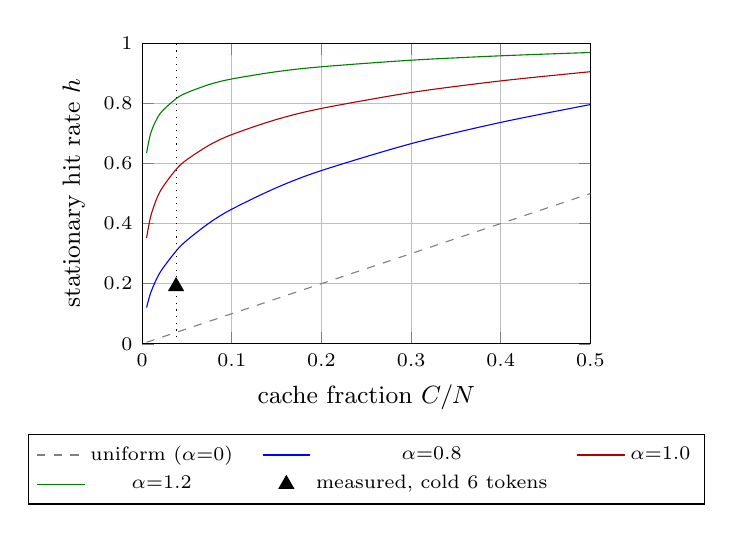
\begin{tikzpicture}
\begin{axis}[width=0.6\textwidth, height=54mm,
  xlabel={cache fraction $C/N$}, ylabel={stationary hit rate $h$},
  xmin=0, xmax=0.5, ymin=0, ymax=1, grid=major,
  legend style={font=\scriptsize, at={(0.5,-0.30)}, anchor=north, legend columns=3,
    /tikz/every even column/.append style={column sep=3mm}},
  tick label style={font=\scriptsize}, label style={font=\small}]
\addplot[gray, dashed] coordinates {(0.005,0.005) (0.5,0.5)};
\addlegendentry{uniform ($\alpha{=}0$)}
\addplot[smooth, blue] coordinates {(0.0050,0.1205) (0.0100,0.1730) (0.0200,0.2370) (0.0379,0.3085) (0.0500,0.3443) (0.0750,0.4021) (0.1000,0.4477) (0.1500,0.5194) (0.2000,0.5762) (0.3000,0.6656) (0.4000,0.7364) (0.5000,0.7957)};
\addlegendentry{$\alpha{=}0.8$}
\addplot[smooth, red!70!black] coordinates {(0.0050,0.3519) (0.0100,0.4283) (0.0200,0.5064) (0.0379,0.5799) (0.0500,0.6125) (0.0750,0.6609) (0.1000,0.6958) (0.1500,0.7462) (0.2000,0.7828) (0.3000,0.8357) (0.4000,0.8744) (0.5000,0.9050)};
\addlegendentry{$\alpha{=}1.0$}
\addplot[smooth, green!50!black] coordinates {(0.0050,0.6342) (0.0100,0.7041) (0.0200,0.7654) (0.0379,0.8152) (0.0500,0.8351) (0.0750,0.8625) (0.1000,0.8808) (0.1500,0.9051) (0.2000,0.9214) (0.3000,0.9432) (0.4000,0.9579) (0.5000,0.9689)};
\addlegendentry{$\alpha{=}1.2$}
\addplot[only marks, mark=triangle*, mark size=3pt, black] coordinates {(0.0379,0.191)};
\addlegendentry{measured, cold 6 tokens}
\draw[dotted] (axis cs:0.0379,0) -- (axis cs:0.0379,1);
\end{axis}
\end{tikzpicture}
\caption{Che-approximation~\citep{che2002hierarchical} LRU hit rate under
Zipf($\alpha$) expert popularity, $N{=}19{,}200$. The dotted line marks our
platform's 727-slot pool ($C/N{=}0.038$); the triangle is the measured
cold-start hit rate, a lower bound on the stationary value.}
\label{fig:che}
\end{figure}

\section{Implementation}\label{sec:impl}

\colistream{} is implemented inside colibr\`i~\citep{colibri2026}: a
${\sim}600$-line CUDA module (slot pool, tile engine, dual copy lanes,
policy, statistics) exporting nine C symbols, plus ${\sim}300$ lines of
engine integration (two-phase submit in the MoE block, the pilot-thread
speculative hook, the RAM-above-VRAM residency probe, host-buffer
page-locking with a budget). On Windows the module ships as a runtime DLL
resolved symbol-by-symbol, so older binaries degrade gracefully; on Linux it
links directly. All settings are command-line flags (\texttt{--stream},
\texttt{--stream-vram}, \texttt{--stream-tile-kb}, \texttt{--stream-pin-gb})
mirrored by environment variables. The engine's existing tiers ---
learned-pin resident experts, RAM LRU, disk container --- are preserved
untouched; \colistream{} slots in between RAM and compute.

\textbf{Correctness methodology.} The full stack is validated
\emph{token-exactly} against a reference \texttt{transformers}
implementation of the same architecture: teacher-forcing 32/32 positions and
greedy generation 20/20 tokens with the tier active, under async disk I/O
and speculative prefetch. A standalone suite covers all four container
formats, odd packed dimensions, eviction pressure, oversized-expert
rejection, two concurrent demand groups, and a prefetch thread racing
demand. As with any change of accumulation order, GPU output is not
bit-identical to the CPU path; greedy argmax ties can therefore fork the
token stream --- every emitted token remains the argmax of a valid forward.

\section{Evaluation}\label{sec:eval}

\textbf{Platform.} RTX 5070 Ti (16\,GB, PCIe 5.0 x16), AVX-512-VNNI CPU,
96\,GB RAM, Windows 11, CUDA 13.1. Model: GLM-5.2~\citep{glm52report}, 744B
parameters, int4 container (370\,GB, 75 MoE layers $\times$ 256 experts,
$k{=}8$, 18.9\,MB/expert), served from an NVMe whose measured cold
random-read bandwidth is $0.49$--$0.51$\,GB/s \emph{regardless of parallelism}
(8/16/32 threads) --- a deliberately adversarial, severely disk-bound
configuration.

\subsection{Microbenchmarks}\label{sec:micro}
Figure~\ref{fig:warm} summarizes the standalone pipeline on GLM-shaped
synthetic experts (11.8\,MB int4, groups of 8, demand path only). Cold
streaming sustains 24.8--27.1\,GB/s with all compute hidden behind the
copies (Theorem~\ref{thm:pipe}'s $\max$ regime: kernels add no wall time);
the warm execution cache serves the same groups kernel-bound at
${\sim}16{,}000$ experts/s with zero PCIe traffic --- a $7.6\times$ gap that
is exactly the replacement-policy ablation of
Proposition~\ref{prop:pollution}: under the frequency-primary score, the
warm pass \emph{re-streamed} every byte (91.9\,ms per 192-expert turnover);
under Eq.~\eqref{eq:score} it hits cache (12.1\,ms).

\begin{figure}[t]
\centering
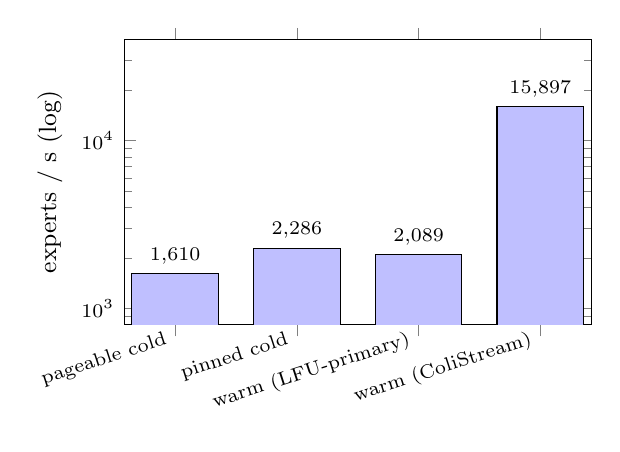
\begin{tikzpicture}
\begin{axis}[width=0.62\textwidth, height=52mm, ybar,
  symbolic x coords={pageable cold, pinned cold, warm (LFU-primary), warm (ColiStream)},
  xtick=data, x tick label style={font=\scriptsize, rotate=18, anchor=east},
  ymode=log, ymin=800, ymax=40000,
  ylabel={experts / s (log)}, label style={font=\small},
  tick label style={font=\scriptsize},
  nodes near coords, point meta=rawy,
  every node near coord/.append style={font=\scriptsize},
  bar width=11mm, enlarge x limits=0.14]
\addplot[fill=blue!25] coordinates {
  (pageable cold,1610) (pinned cold,2286) (warm (LFU-primary),2089) (warm (ColiStream),15897)};
\end{axis}
\end{tikzpicture}
\caption{Standalone throughput, 192 GLM-shaped experts in groups of 8
(2\,MB tiles). ``Warm (LFU-primary)'' is the pre-fix policy of
Proposition~\ref{prop:pollution}: a full working-set turnover polluted the
cache and every ``warm'' pass re-streamed at PCIe speed; the recency-primary
policy serves it from VRAM, $7.6\times$ faster and with zero bus traffic.}
\label{fig:warm}
\end{figure}

\subsection{End-to-end on the 744B model}
We compare the engine's optimized CPU expert path (AVX-512-VNNI kernels,
async I/O pool) against \colistream{} on identical settings: same prompt,
greedy decoding, 16 tokens, speculation disabled on both sides, learned pin
disabled, runs interleaved with controls to bound page-cache drift (CPU
controls before and after the streamed run agree within 0.5\%).

\begin{table}[h]
\centering\small
\begin{tabular}{lccccc}
\toprule
configuration & wall (s) & disk (s) & expert compute (s) & loads/token & tok/s \\
\midrule
CPU path, default flags$^\dagger$ & 386.1 & 370.3 & 10.2 & 1216.5 & 0.041 \\
CPU path, fair (\texttt{DRAFT=0}) & 277.3 & 264.2 & 8.5 & 750.0 & 0.058 \\
\colistream{} & \textbf{260.3} & 223.2 & 32.3$^\ddagger$ & 750.0 & \textbf{0.061} \\
\bottomrule
\end{tabular}
\caption{End-to-end A/B, cold-ish cache. $^\dagger$Confounded: without CUDA
the engine defaults speculative decoding on, which on a cold cache inflates
expert traffic $1.6\times$ --- an A/B that ignores this reports a misleading
$1.48\times$ advantage. $^\ddagger$Includes the GPU pipeline's synchronization
window, largely overlapped with disk service.}
\label{tab:ab}
\end{table}

\begin{figure}[t]
\centering
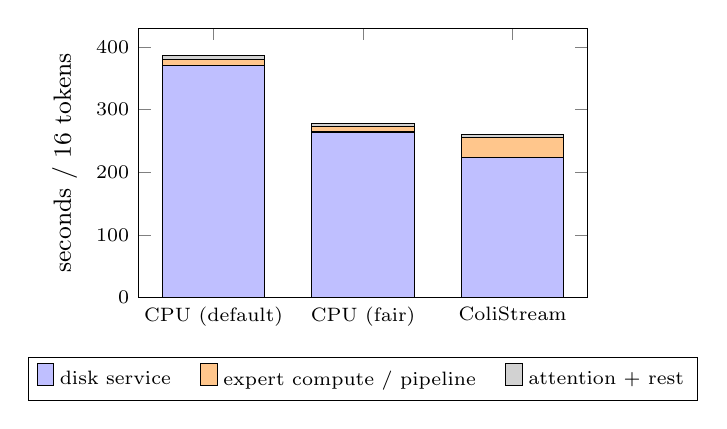
\begin{tikzpicture}
\begin{axis}[width=0.6\textwidth, height=50mm, ybar stacked,
  symbolic x coords={CPU (default), CPU (fair), ColiStream},
  xtick=data, ymin=0, ymax=430, ylabel={seconds / 16 tokens},
  bar width=13mm, enlarge x limits=0.25,
  legend style={font=\scriptsize, at={(0.5,-0.22)}, anchor=north, legend columns=3,
    /tikz/every even column/.append style={column sep=3mm}},
  tick label style={font=\scriptsize}, label style={font=\small}]
\addplot[fill=blue!25] coordinates {(CPU (default),370.3) (CPU (fair),264.2) (ColiStream,223.2)};
\addlegendentry{disk service}
\addplot[fill=orange!45] coordinates {(CPU (default),10.2) (CPU (fair),8.5) (ColiStream,32.3)};
\addlegendentry{expert compute / pipeline}
\addplot[fill=gray!35] coordinates {(CPU (default),5.6) (CPU (fair),4.6) (ColiStream,4.8)};
\addlegendentry{attention + rest}
\end{axis}
\end{tikzpicture}
\caption{Wall-time decomposition of Table~\ref{tab:ab}. The workload is
disk-dominated ($\varphi = 0.95$); \colistream's win comes from removing
expert compute from the critical path \emph{and} from deeper disk/transfer
overlap, together slightly exceeding the compute-only Amdahl ceiling.}
\label{fig:ab}
\end{figure}

\colistream{} is $1.065\times$ faster on a workload whose disk fraction is
$\varphi = 264.2/277.3 = 0.953$. By Corollary~\ref{cor:speedup}, eliminating
expert compute \emph{entirely} could yield at most $1/\varphi = 1.049\times$;
the additional margin comes from reduced disk service time (223\,s vs.\
264\,s at identical 750 loads/token), i.e.\ deeper overlap of preads with
the GPU pipeline once CPU cores stop competing with the I/O pool. Two
honesty notes. First, Table~\ref{tab:ab}'s top row shows how easily this
comparison is inflated: engine defaults enable speculative
decoding~\citep{leviathan2023fast} only on the CPU side, and on a cold cache
each verified draft routes extra experts (1216 vs.\ 750 loads/token), so a
naive A/B credits \colistream{} with $1.48\times$. Second, greedy paths can
fork between kernel families (accumulation order), so per-run cache
statistics are indicative, not paired.

The pilot prefetch (source 2) composes as designed: with cross-layer
prediction active, speculative uploads land in the execution cache and are
consumed by demand before eviction, at zero measured cost to demand latency
(Proposition~\ref{prop:tile}'s window).

\subsection{Where the architecture pays}
Corollary~\ref{cor:speedup} predicts the regimes. On this platform the disk
is $50\times$ slower than the link, so cold decode saturates the NVMe and
\emph{any} expert-compute change is bounded by $1.05\times$ --- which
\colistream{} meets and slightly exceeds. On the same box with a
page-cache-warm or RAM-resident expert set, the binding stage becomes
$\max(\beta_2, \beta_3)$: the streamed pipeline's 2{,}250 experts/s cold and
${\sim}16{,}000$ experts/s warm against 600 expert-loads/token give ceilings
of 3.7 and 26 tok/s respectively, versus a CPU expert path that our
measurements place at ${\sim}8.5$\,s per 12{,}000 applications
(${\sim}1{,}400$ experts/s) --- a $1.6$--$11\times$ compute-side advantage
that materializes exactly as the storage bottleneck is relieved (faster
NVMe, larger RAM, higher $h_V$ via Eq.~\eqref{eq:che}).

\section{Limitations and Future Work}
Single-GPU only; multi-device streaming with expert placement across links
is open. In-flight copies cannot be cancelled --- tile granularity bounds
but does not eliminate speculative interference. The Windows/WDDM submission
path caps $B_\infty$ at 27.6\,GB/s on a 64\,GB/s link; a Linux/native
port of the measurement is future work. The execution cache stores whole
experts; caching \emph{tiles} would admit partial residency and adaptive
precision (int1.5/int1 re-quantization for cold experts) at the cost of a
two-level directory. Finally, our hit-rate analysis assumes an independent
reference model; routing is in fact autocorrelated (which helps), and a
Markov-modulated analysis would tighten \S\ref{sec:che}.

\section{Conclusion}
\colistream{} reframes MoE offloading: stop asking what fits in VRAM, and
instead keep every engine of the memory hierarchy busy on a single stream of
expert tiles. The mathematics is classical --- pipeline bounds, cache
approximations, Amdahl's law --- but their composition yields a design in
which correctness never depends on prediction, interference is provably
tile-bounded, and performance degrades to exactly the bottleneck the
hardware imposes. On a 16\,GB consumer GPU the architecture streams a 744B
model's experts at effective link speed, serves repeats at
$16{,}000$ experts/s from cache, and beats a heavily optimized CPU path even
on a workload constructed so that almost nothing was winnable. The gap
between that workload's $1.065\times$ and the warm regime's $11\times$
compute advantage is not a promise; it is a disk upgrade.

\paragraph{Acknowledgments.} This work builds on the colibr\`i engine
\citep{colibri2026}; the resident tier, learned pinning, and router-lookahead
measurement infrastructure are its author's.

\bibliographystyle{plainnat}
\bibliography{colistream}

\end{document}
